\documentclass[hidelinks,12pt]{article}
\usepackage[left=0.25cm,top=1cm,right=0.25cm,bottom=1cm]{geometry}
%\usepackage[landscape]{geometry}
\textwidth = 20cm
\hoffset = -1cm
\usepackage[utf8]{inputenc}
\usepackage[spanish,es-tabla, es-lcroman]{babel}
\usepackage[autostyle,spanish=mexican]{csquotes}
\usepackage[tbtags]{amsmath}
\usepackage{nccmath}
\usepackage{amsthm}
\usepackage{amssymb}
\usepackage{mathrsfs}
\usepackage{graphicx}
\usepackage{subfig}
\usepackage{caption}
%\usepackage{subcaption}
\usepackage{standalone}
\usepackage[outdir=./Imagenes/]{epstopdf}
\usepackage{siunitx}
\usepackage{physics}
\usepackage{color}
\usepackage{float}
\usepackage{hyperref}
\usepackage{multicol}
\usepackage{multirow}
%\usepackage{milista}
\usepackage{anyfontsize}
\usepackage{anysize}
%\usepackage{enumerate}
\usepackage[shortlabels]{enumitem}
\usepackage{capt-of}
\usepackage{bm}
\usepackage{mdframed}
\usepackage{relsize}
\usepackage{placeins}
\usepackage{empheq}
\usepackage{cancel}
\usepackage{pdfpages}
\usepackage{wrapfig}
\usepackage[flushleft]{threeparttable}
\usepackage{makecell}
\usepackage{fancyhdr}
\usepackage{tikz}
\usepackage{bigints}
\usepackage{menukeys}
\usepackage{tcolorbox}
\tcbuselibrary{breakable}
\usepackage{scalerel}
\usepackage{pgfplots}
\usepackage{pdflscape}
\pgfplotsset{compat=1.16}
\spanishdecimal{.}
\renewcommand{\baselinestretch}{1.5} 
\renewcommand\labelenumii{\theenumi.{\arabic{enumii}})}

\newcommand{\python}{\texttt{python}}
\newcommand{\textoazul}[1]{\textcolor{blue}{#1}}
\newcommand{\azulfuerte}[1]{\textcolor{blue}{\textbf{#1}}}
\newcommand{\funcionazul}[1]{\textcolor{blue}{\textbf{\texttt{#1}}}}

\newcommand{\pderivada}[1]{\ensuremath{{#1}^{\prime}}}
\newcommand{\sderivada}[1]{\ensuremath{{#1}^{\prime \prime}}}
\newcommand{\tderivada}[1]{\ensuremath{{#1}^{\prime \prime \prime}}}
\newcommand{\nderivada}[2]{\ensuremath{{#1}^{(#2)}}}


\newtheorem{defi}{{\it Definición}}[section]
\newtheorem{teo}{{\it Teorema}}[section]
\newtheorem{ejemplo}{{\it Ejemplo}}[section]
\newtheorem{propiedad}{{\it Propiedad}}[section]
\newtheorem{lema}{{\it Lema}}[section]
\newtheorem{cor}{Corolario}
\newtheorem{ejer}{Ejercicio}[section]

\newlist{milista}{enumerate}{2}
\setlist[milista,1]{label=\arabic*)}
\setlist[milista,2]{label=\arabic{milistai}.\arabic*)}
\newlength{\depthofsumsign}
\setlength{\depthofsumsign}{\depthof{$\sum$}}
\newcommand{\nsum}[1][1.4]{% only for \displaystyle
    \mathop{%
        \raisebox
            {-#1\depthofsumsign+1\depthofsumsign}
            {\scalebox
                {#1}
                {$\displaystyle\sum$}%
            }
    }
}
\def\scaleint#1{\vcenter{\hbox{\scaleto[3ex]{\displaystyle\int}{#1}}}}
\def\scaleoint#1{\vcenter{\hbox{\scaleto[3ex]{\displaystyle\oint}{#1}}}}
\def\scaleiiint#1{\vcenter{\hbox{\scaleto[3ex]{\displaystyle\iiint}{#1}}}}
\def\bs{\mkern-12mu}

\newcommand{\Cancel}[2][black]{{\color{#1}\cancel{\color{black}#2}}}



\title{\vspace{-2cm} Lista de ejercicios a cuenta \\ {\large Curso Física Computacional} \vspace{-3ex}}
\author{M. en C. Gustavo Contreras Mayén. \texttt{gux7avo@ciencias.unam.mx}}
\date{}

\begin{document}

\fontsize{14}{14}\selectfont
\vspace{-4cm}
\maketitle


\section{Tema 1.}


\section{Tema 2.}

\subsection{Diferenciación.}

\begin{enumerate}
\item Demuestra que la aproximación a la derivada por diferencias hacia adelante de orden $\order{h^{2}}$ es:
\begin{align*}
\pderivada{f} (x) = \dfrac{- 3 f (x) \, + 4 \, f (x + h) - f (x + 2 \, h)}{2 \, h}
\end{align*}
\item Demuestra que a la derivada por diferencias hacia atrás de orden $\order{h^{2}}$ es::
\begin{align*}
\pderivada{f} (x) = \dfrac{3 \, f (x) \, - 4 \, f (x + h) + f (x + 2 \, h)}{2 \, h}
\end{align*}
\item Del ejercicio del mecanismo articulado, obtener las tres gráficas:
\begin{enumerate}[label=\roman*)]
\item Puntos de velocidad angular $\dot{\beta}$ de la tabla.
\item Nuevos puntos interpolados, ocupando interpolación de Lagrange, Newton o del módulo \texttt{numpy} o \texttt{scipy}.
\item Una curva de interpolación con \texttt{scipy}.
\end{enumerate}
\begin{figure}[H]
    \centering
    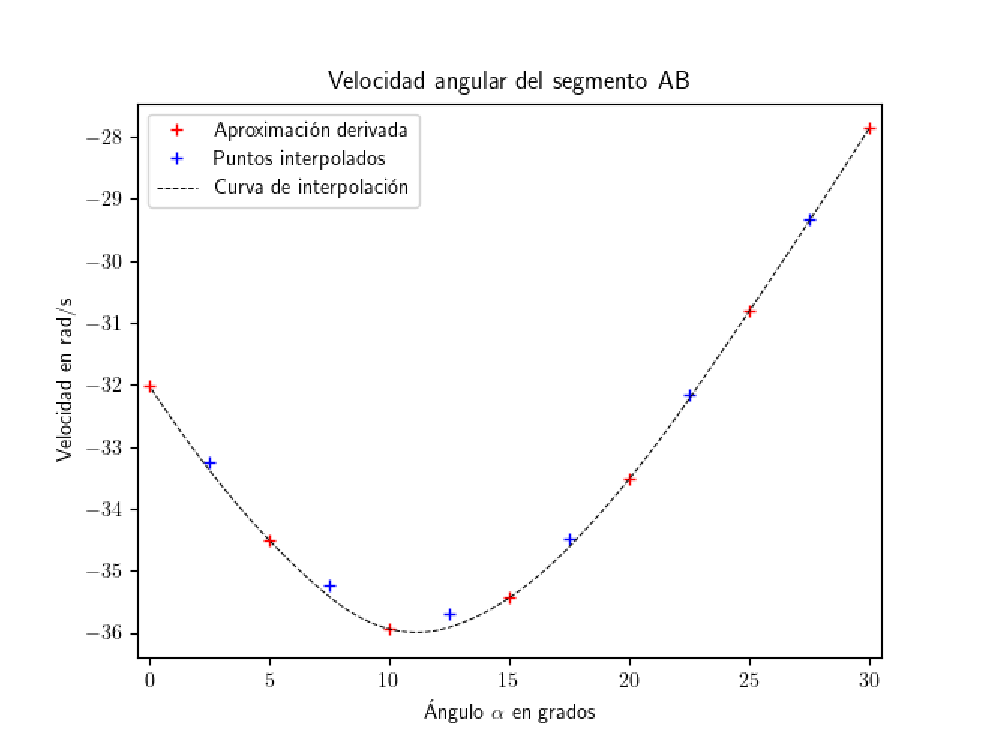
\includegraphics[scale=0.55]{Imagenes/diferenciacion_ejercicio_segmento_03.eps}
    \caption{Esta sería la tercera gráfica que conjunta los tres puntos pedidos del ejercicio de los segmentos articulados.}
\end{figure}
\item Del ejercicio del circuito $RL$, obtener las tres gráficas:
\begin{enumerate}[label=\roman*)]
\item Voltajes para los tiempos indicados en la tabla.
\item Nuevos puntos interpolados, ocupando interpolación de Lagrange, Newton o del módulo \texttt{numpy} o \texttt{scipy}.
\item Una curva de interpolación con \texttt{scipy}.
\end{enumerate}
\begin{figure}
    \centering
    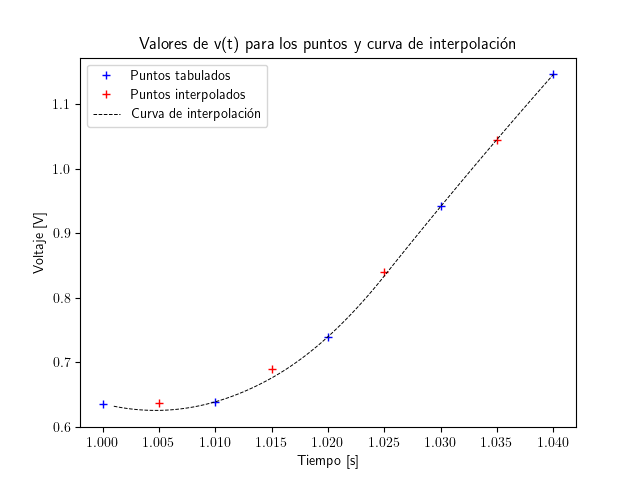
\includegraphics[scale=0.55]{Imagenes/diferenciacion_ejercicio_RL_03.png}
    \caption{Esta sería la tercera gráfica que conjunta los tres puntos pedidos para el ejercicio del circuito $RL$.}
\end{figure}

\end{enumerate}


\end{document}